\documentclass[11pt]{article}
\usepackage[utf8]{inputenc}
\usepackage[french]{babel}
\usepackage[margin=3cm, paperwidth=21cm, paperheight=29.7cm]{geometry}
\usepackage{graphicx}
\usepackage{SIunits}
\usepackage{tabto}
\usepackage{eurosym}
\usepackage{subcaption}
\usepackage{hyperref}
\hypersetup{hidelinks}
\usepackage{url}
\usepackage{listings}
\usepackage[footnote]{acronym}
\usepackage[T1]{fontenc}
\usepackage{array}
\usepackage{titlesec}
\usepackage{todonotes}

\usepackage{fancyhdr}
\usepackage{caption}

\usepackage{xcolor}
 
\definecolor{codegreen}{rgb}{0,0.6,0}
\definecolor{codegray}{rgb}{0.5,0.5,0.5}
\definecolor{codepurple}{rgb}{0.58,0,0.82}
\definecolor{backcolour}{rgb}{0.95,0.95,0.92}
\definecolor{bluekeywords}{rgb}{0.13,0.13,1}
\definecolor{greencomments}{rgb}{0,0.5,0}
\definecolor{redstrings}{rgb}{0.9,0,0}
\definecolor{typedef}{rgb}{0.227, 0.49, 0.49}
\definecolor{violet}{rgb}{0.255, 0.2588, 0.5333}
\lstdefinestyle{C_Style}{
    language=C,
    backgroundcolor=\color{backcolour},   
    commentstyle=\color{codegreen},
    keywordstyle=\color{bluekeywords},
    numberstyle=\tiny\color{codegray},
    stringstyle=\color{codepurple},
    basicstyle=\ttfamily\footnotesize,
    breakatwhitespace=false,         
    breaklines=true,                 
    captionpos=b,                    
    keepspaces=true,                 
    numbers=left,                    
    numbersep=5pt,                  
    showspaces=false,                
    showstringspaces=false,
    showtabs=false,                  
    tabsize=2,
    emph={%  
    __mavlink_custom_struct_t, uint8_t, uint16_t, uint32_t, uint64_t, mavlink_custom_struct_t%
    },emphstyle={\color{typedef}}%
}

\lstdefinestyle{XML_Style}{
  language=XML,
  backgroundcolor=\color{backcolour},   
  commentstyle=\color{codegreen},
  keywordstyle=\color{bluekeywords},
  numberstyle=\tiny\color{codegray},
  stringstyle=\color{codepurple},
  basicstyle=\ttfamily\footnotesize,
  breakatwhitespace=false,         
  breaklines=true,                 
  captionpos=b,                    
  keepspaces=true,                 
  numbers=left,                    
  numbersep=5pt,                  
  showspaces=false,                
  showstringspaces=false,
  showtabs=false,                  
  tabsize=2,
  morekeywords={mavlink, message, enums, messages, wip, field, description, dialect, include},
  emph={  
    type, id, name, enum
    },emphstyle={\color{violet}}
}

\lstset{style=C_Style}
\pagestyle{fancy}
\lhead{Tachyssema} % controls the left corner of the header
\chead{} % controls the center of the header
\rhead{V200221} % controls the right corner of the header
\lfoot{} % controls the left corner of the footer
\cfoot{Page~\thepage} % controls the center of the footer
\rfoot{} % controls the right corner of the footer
\renewcommand{\headrulewidth}{0.4pt}
\renewcommand{\footrulewidth}{0.4pt}

\titleclass{\subsubsubsection}{straight}[\subsection]

\newcounter{subsubsubsection}[subsubsection]
\renewcommand\thesubsubsubsection{\thesubsubsection.\arabic{subsubsubsection}}
\renewcommand\theparagraph{\thesubsubsubsection.\arabic{paragraph}} % optional; useful if paragraphs are to be numbered


\titleformat{\subsubsubsection}
  {\normalfont\normalsize\bfseries}{\thesubsubsubsection}{1em}{}
\titlespacing*{\subsubsubsection}
{0pt}{3.25ex plus 1ex minus .2ex}{1.5ex plus .2ex}
\makeatletter

\titleclass{\subsubsubsubsection}{straight}[\subsection]

\newcounter{subsubsubsubsection}[subsubsubsection]
\renewcommand\thesubsubsubsubsection{\thesubsubsubsection.\arabic{subsubsubsubsection}}

\titleformat{\subsubsubsubsection}
  {\normalfont\normalsize\bfseries}{\thesubsubsubsubsection}{1em}{}
\titlespacing*{\subsubsubsubsection}
{0pt}{3.25ex plus 1ex minus .2ex}{1.5ex plus .2ex}
\makeatletter

\renewcommand\paragraph{\@startsection{paragraph}{6}{\z@}%
  {3.25ex \@plus1ex \@minus.2ex}%
  {-1em}%
  {\normalfont\normalsize\bfseries}}
\renewcommand\subparagraph{\@startsection{subparagraph}{7}{\parindent}%
  {3.25ex \@plus1ex \@minus .2ex}%
  {-1em}%
  {\normalfont\normalsize\bfseries}}
\def\toclevel@subsubsubsection{4}
\def\toclevel@subsubsubsubsection{5}
\def\toclevel@paragraph{6}
\def\toclevel@paragraph{7}
\def\l@subsubsubsection{\@dottedtocline{4}{7em}{4em}}
\def\l@subsubsubsubsection{\@dottedtocline{5}{10em}{5em}}
\def\l@paragraph{\@dottedtocline{6}{13em}{6em}}
\def\l@subparagraph{\@dottedtocline{7}{17em}{7em}}
\makeatother

\setcounter{secnumdepth}{5} % Profondeur des nombres des titres
\setcounter{tocdepth}{3}

\renewcommand{\contentsname}{Table des matières}
\begin{document}
\thispagestyle{plain}% Removes the header from the first page. Change plain to empty to remove the numbering entirely.

\begin{titlepage}

  \newcommand{\HRule}{\rule{\linewidth}{0.5mm}} % Defines a new command for the horizontal lines, change thickness here
  
  \center % Center everything on the page
   
  %----------------------------------------------------------------------------------------
  %	HEADING SECTIONS
  %----------------------------------------------------------------------------------------
  
  %\textsc{\LARGE University Name}\\[1.5cm] % Name of your university/college
  %\textsc{\Large Major Heading}\\[0.5cm] % Major heading such as course name
  %\textsc{\large Minor Heading}\\[0.5cm] % Minor heading such as course title
  
  %----------------------------------------------------------------------------------------
  %	TITLE SECTION
  %----------------------------------------------------------------------------------------
  
  \HRule \\[0.4cm]
  { \huge \bfseries Rapport \textsc Alternance Master SME  }\\[0.4cm] % Title of your document
  { \LARGE Première année}\\[0.4cm] % Title of your document
  \HRule \\[1.5cm]
   

  %----------------------------------------------------------------------------------------
  %	AUTHOR SECTION
  %----------------------------------------------------------------------------------------
  
  %\begin{minipage}{0.4\textwidth}
  %\begin{flushleft} \large
  %\emph{Author:}\\
  %John \textsc{Smith} % Your name
  %\end{flushleft}
  %\end{minipage}
  %~
  %\begin{minipage}{0.4\textwidth}
  %\begin{flushright} \large
  %\emph{Supervisor:} \\
  %Dr. James \textsc{Smith} % Supervisor's Name
  %\end{flushright}
  %\end{minipage}\\[2cm]
  
  % If you don't want a supervisor, uncomment the two lines below and remove the section above
  \Large
  Etudiant : Cyprien \textsc{Quivet}\\ % Your name
  \Large
  Tuteur : Nicolas  \textsc{Roddier}\\ % Your name
  
  %----------------------------------------------------------------------------------------
  %	DATE SECTION
  %----------------------------------------------------------------------------------------
  
  
  %----------------------------------------------------------------------------------------
 % \vfill % Fill the rest of the page with whitespace
  %	LOGO SECTION
  %----------------------------------------------------------------------------------------


  \begin{figure}[b]
    \centering
    
\includegraphics{img/LogoTachyssema.png}\\[1cm] % Include a department/university logo - this will require the graphicx package
    \label{fig:LogoTachyssema}
  \end{figure}
  {\Large Avril 2020}\\[2cm] % Date, change the \today to a set date if you want to be precise

  
   
  %----------------------------------------------------------------------------------------
  
  \end{titlepage}
\newpage
\setcounter{page}{2}

\renewcommand{\thepage}{\arabic{page}}

\tableofcontents
\newpage

\section{Tachysséma Développement}
\subsection{Présentation de la Société}

Dans le cadre du master SME, je réalise ma première année d'alternance au sein de la SARL TACHYSSEMA DEVELOPPEMENT basée à Labège (31).
Cette société est spécialisée dans le traitement vidéo et le traitment du signal en temps réel pour des systèmes éléctroniques embarqués. 

En conséquence, la société possède un rayon d'action étendu qui comprend de la R\&D, du développement matériel (caméras embarqués, conception de cartes éléctroniques) et du dévellopement logiciel. 

Les domaines d'applications de la société est également varié puisque la société peut être amenée à réaliser des projet en lien avec l'aéronotique, le secteur médical, militaire ou encore automobile. 



\subsection{Organisation interne}

Les locaux de Tachysséma Développement sont partagés avec Visif Technology, une société spécialisée dans le dévellopement de solutions technologiques pour les énergies renouvelables. Cependant les deux sociétés possèdes des projets communs et travaillent ensembles. 

Au sein de Tachysséma Développement, Nicolas Roddier, mon tuteur d'alternance et gérant de la société est assité par un ingénieur en automatique ainsi qu'une stagiaire M2 SME, un alternant en M2 SME et moi même. 

Pour Visif Technology, sont présents 

Il 



\newpage

\section{Projets Réalisés}
Dans cette partie nous réaliserons la synthése des projets principaux menés depuis mon arrivé chez Tachysséma Développement, en octobre 2019. 

\subsection{Réalisation d'une IHM avec l'environnement GTK}

Dans le cadre d'un projet de gestion et contrôle de pixels deffectueux présents sur un capteur d'une caméra, j'ai réalisé une interface homme machine permettant de réaliser l'interface entre l'utilisateur et un module FPGA qui contrôle le capteur d'une caméra. 
\\ 

\subsubsection{Contexte} 

Le capteur d'une caméra est constitué d'un ensemble pixels qui captent la lumière entrante. On peut représenter l'ensemble de ces pixels sous la forme d'une matrice. Avec le temps, il est possible que certains pixels deviennent deffectueux, on parle alors de pixels morts. Les pixels deffectueux doivent pouvoir être localisés, corigés ou remplacés.  
\newline

La caméra est composée d'un FPGA qui contrôle le capteur vidéo. Il permet notament de réaliser le traitement des pixels deffectueux. L'interface homme machine interragit avec le FPGA, elle permettra la réalisations des actions de lectures et d'écriture dans une mémoire EEPROM qui contient les coordonnés matricielle des pixels morts. 

\subsubsection{Cahier des charges de l'IHM } 

\begin{figure}[ht]
	\centering
    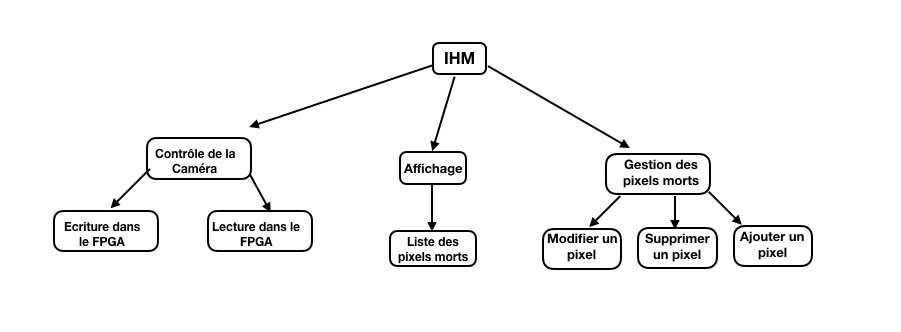
\includegraphics[scale=0.5]{img/cdcIHM.png}
    \caption{Générateur MAVGEN}
    \label{fig:mavgen}
\end{figure}

Voici ci-dessous les principales fonctions qui sont réalisées par l'IHM : 
\newline
\begin{itemize}
	\item L'utilisateur peut lire et écrire la liste des pixels déffectueux dans un fichier .txt qui est sauvegardé sur le disque dur de l'ordinateur (ou est executée l'IHM). 
	\item La matrice
	\item L'IHM peut intérragir avec la caméra par le biais d'une communication série. Elle réalise des opérations de lectures et d'écritures dans une table FPGA ainsi que dans une mémoire EEPROM qui contient les coordonnées des pixels défectueux. 
	\item Une fois que les coordonnés des pixels morts sont chargés de la caméra vers l'IHM ou du fichier .txt vers l'IHM, cette dernière les affiches sous la forme d'une liste comportant deux colonnes (une pour la ligne et une pour la colonne du pixel mort). 
	\item L'utilisateur peut effectuer différentes actions sur la liste des mauvais pixels. Il peut notament ajouter, supprimer ou remplacer des pixels deffectueux. A chaque modification, la liste est actualisée et transmise au FPGA.

\end{itemize}

\subsubsection{Implémentation}

\begin{figure}[ht]
    \centering
    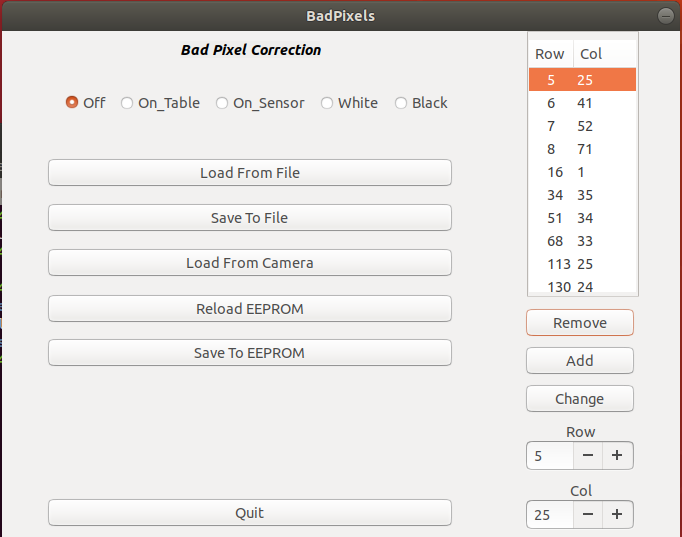
\includegraphics[scale=0.45]{img/IHM.png}
    \caption{Apperçu de l'IHM}
    \label{fig:CameraCmdsettings}
\end{figure}

\subsubsubsection{Interface graphique}

La première étape que j'ai effectué sur ce projet est la réalisation de la partie graphique de l'IHM. Cette dernière devait s'éxecuter sur une distribution linux.

En conséquence j'ai utilisé l'outil de développement graphique Glade qui intègre GTK+. Glade permet facilité la réalisation d'interface graphique: En effet on vient placer les différents objets ( boutons, champs de texte, curseurs etc .. ) sans passer par le code. 

Une fois ce processus terminé, glade génrère la solution obtenu dans un fichier .XML que nous pouvons intégrer directement dans un langage de programmation ( C, C++, Pyhton et d'autres encore). 
\newline

\subsubsubsection{Implémentation du code}

Ensuite j'ai pu implémenté le code en langage C ce qui permet d'établir un lien entre un évement lié à l'interface graphique ( appuie sur un bouton, changement de valeur sur un curseur ..) et une fonction répondant au cahier des charges ( envoie des données dans le FPGA, quitter l'IHM ou encore écrire le fichier .txt par exemple). 



\subsection{Projet WindFloat Atlantic : Traitement des données d'un capteur}

\begin{figure}[ht]
    \centering
    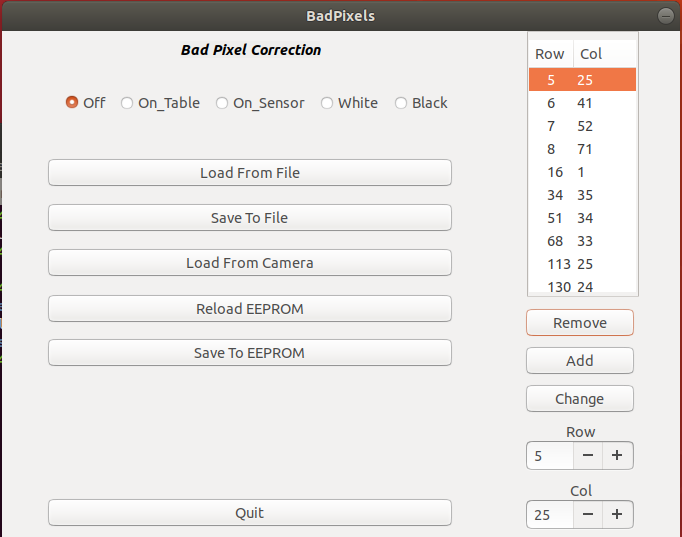
\includegraphics[scale=0.45]{img/IHM.png}
    \caption{Apperçu de l'IHM}
    \label{fig:CameraCmdsettings}
\end{figure}

\subsubsection{Contexte}

\subsubsubsection{Le projet WindFloat Atlantic}



Pour ce faire la commande MAV\_CMD\_VIDEO\_STOP\_STREAMING est transmise à la caméra et la diffusion vidéo est stoppée si l'acquittement émit par la caméra correspond à MAV\_RESULT\_ACCEPTED.
\newpage

\section{Personnalisation du protocole MAVLINK }

Il est possible de créer des messages dont les paramètres sont personnalisés par l'utilisateur. L'intérêt est de pouvoir échanger des données qui ne sont pas incluses dans les messages existants en utilisant tout de même le protocole MAVLINK. 
\subsection{Solution envisageable }
Les messages MAVLINK sont définis dans des fichiers .XML nommés dialectes. Le dialecte "Common.xml" contient la définition de tous les principaux messages du protocole MAVLINK. Cependant pour des applications spécifiques, d'autres dialectes ont été crées. 
C'est par exemple le cas du dialecte "ArdupilotMega.xml" crée par la suite logiciel de pilotage automatique de véhicule sans pilote Ardupilot.\newline

Une fois les messages personnalisés ajoutés dans les dialectes, il faut pouvoir les générer dans un langage de programmation pour les implémenter. Pour ce faire il existe l'outil MAVGEN qui permet de générer en langage C, C++, Java et Python les dialectes crées.\newline

Lorsque les dialectes sont générés, il faut inclure les fichiers sources au projet. Il est alors possible d'échanger les nouveau messages via le protocole MAVLINK. 
\subsection{Exemple}
\subsubsection{Création d'un dialecte}
Nous voulons échanger un nouveau message MAVLINK contenant les 4 paramètres suivants :
\begin{flushleft}
	$var1$, $var2$, $var3$, $var4$, qui sont des entiers non signés sur 32 bits.
\end{flushleft}

La première étape est donc de créer un nouveau dialecte que l'on nommera "tachyssema.xml" et qui contiendra la définition du nouveau message personnalisé. (voir figure ci-dessous).
\lstset{style=XML_Style}
\begin{lstlisting}[caption={Nouveau dialecte},captionpos=b, label={lst:custom_dialect_def}]
<?xml version="1.0"?>
<mavlink>
	<include>common.xml</include>
	<!-- <version>9</version> -->
	<enums>
	</enums>
	<messages>
		<message id="402" name="Custom_Struct">
			<wip/>
			<description>MESSAGE PERSONNALISE TEST</description>
				<field type="uint32_t" name="var1" enum="variable">Comment variable 1</field>
				<field type="uint32_t" name="var2" enum="variable">Comment variable 2</field>
				<field type="uint32_t" name="var3" enum="variable">Comment variable 3</field>
				<field type="uint32_t" name="var4" enum="variable">Comment variable 4</field>
		</message>
	</messages>
</mavlink>
\end{lstlisting}
 \subsubsection{Génération de la librairie en langage C }
 A présent, il faut généré le dialecte crée en un fichier exploitable en langage C. Pour ce faire, on ouvre le générateur de librairie MAVGEN comme sur la figure ci-dessous : 
\begin{figure}[ht]
	\centering
    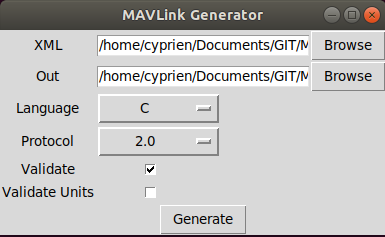
\includegraphics[scale=0.75]{img/mavgen.png}
    \caption{Générateur MAVGEN}
    \label{fig:mavgen}
\end{figure}
Le GUI permet de choisir le fichier source, le repertoire cible ainsi que le langage et la version de MAVLINK désirée. 
Une fois la génération terminée en langage C, on retrouve nos fichiers au sein de la librairie MAVLINK : 
\begin{figure}[ht]
	\centering
    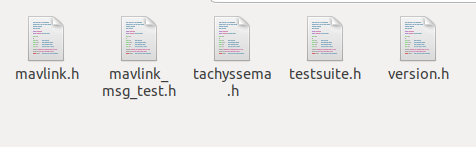
\includegraphics[scale=0.5]{img/fichiersC.png}
    \caption{Fichiers .C générés }
    \label{fig:mavgen}
\end{figure}
\subsubsection{Utilisation du message dans un projet}
A présent, il est possible de  transmettre le nouveau message via le protocole MAVLINK. On retrouve bien dans les fichiers générés la structure de notre message: 
\lstset{style=C_Style}
\begin{lstlisting}[caption={Structure personnalisée},captionpos=b, label={lst:custom_struct __mavlink_message_test_t}]
MAVPACKED(
	typedef struct __mavlink_custom_struct_t {
		uint32_t var1; /*<  Comment variable 1*/
		uint32_t var2; /*<  Comment variable 2*/
		uint32_t var3; /*<  Comment variable 3*/
		uint32_t var4; /*<  Comment variable 4*/
	}) mavlink_custom_struct_t;
\end{lstlisting}


\newpage
\section{Mise en œuvre du protocole MAVLINK pour le système OptSys}
\subsection{Utilisation des fonctions incluses dans le protocole MAVLINK}
\subsubsection{Heartbeat}
Il faudra utiliser l'échange Heartbeat précédemment décrit pour s'assurer que la caméra est bien connectée au réseau. Il reste cependant à définir à quelle période ce type de message doit être émit par la caméra pour la considérer connectée ou non au réseau.
\subsubsection{Informations et paramètres de la caméra}
Pour obtenir les informations de la caméra, l’échange « Camera informations » sera établit et permettra à la caméra de transmettre la structure de données « CAMERA
\_INFORMATIONS » renvoyant l’ensemble des paramètres présents sur la figure 2.

\

Les messages MAV\_CMD\_REQUEST\_CAMERA\_SETTINGS et MAV\_CMD\_SET
\_CAMERA\_MODE permettront d’obtenir et/ou modifier les paramètres suivants :
\begin{itemize}
	\item Le zoom de la caméra
	\item Le focus de la caméra
	\item Le mode dans lequel se trouve la caméra (prise d’image ou de vidéo)

\end{itemize}


\subsubsection{Lancement et arrêt d'une diffusion vidéo}

Pour activer la diffusion vidéo de la caméra, nous utiliserons la commande MAV
\_CMD\_VIDEO\_START\_STREAMING.
\newline 
\par
    Pour arrêter  la diffusion vidéo de la caméra, nous utiliserons la commande MAV
\_CMD\_VIDEO\_STOP\_STREAMING.

\subsection{Ajout de fonctions publiques au protocole MAVLINK}

La création d’un dialecte publique sera mis en œuvre pour ajouter des définitions de messages publiques non existants via le protocole MAVLINK qui seront utiles à la caméra.
Par exemple l'ajout de messages pour gérer la saturation et la teinte de la vidéo. 

\subsection{Ajout de fonctions privées au protocole MAVLINK}

Certains attributs de la caméra ne seront pas visibles par le client. Comme par exemple :  
\begin{itemize}
	\item L'offset
	\item La matrice
	\item Le seuil  
	\item La colorimétrie
	\item Le numéro de série etc ..

\end{itemize}
\

Pour se faire, un dialecte privé contentant la définition de ces messages sera établit. 



\clearpage

\end{document}